\documentclass{sigplanconf}

\usepackage{lgrind}
\usepackage[dvips]{graphicx}
\usepackage{verbatim}
\pagestyle{plain}

%% This bit allows you to either specify only the files which you wish to
%% process, or `all' to process all files which you \include.
%% Krishna Sethuraman (1990).

\typein [\files]{Enter file names to process, (chap1,chap2 ...), or `all' to
process all files:}
\def\all{all}
\ifx\files\all \typeout{Including all files.} \else \typeout{Including only \files.} \includeonly{\files} \fi

\begin{document}

% -*-latex-*-

\title{Linear State-Space Analysis and Optimization of StreamIt Programs}

\author{Sitij Agrawal}
\department{Department of Electrical Engineering and Computer Science}
% If the thesis is for two degrees simultaneously, list them both
% separated by \and like this:
% \degree{Doctor of Philosophy \and Master of Science}
\degree{Master of Engineering in Computer Science and Engineering}
\degreemonth{August}
\degreeyear{2004}
\thesisdate{August 26, 2004}

%% By default, the thesis will be copyrighted to MIT.  If you need to copyright
%% the thesis to yourself, just specify the `vi' documentclass option.  If for
%% some reason you want to exactly specify the copyright notice text, you can
%% use the \copyrightnoticetext command.
%\copyrightnoticetext{\copyright IBM, 1990.  Do not open till Xmas.}

% If there is more than one supervisor, use the \supervisor command
% once for each.
\supervisor{Saman Amarasinghe}{Associate Professor}

% This is the department committee chairman, not the thesis committee
% chairman.  You should replace this with your Department's Committee
% Chairman.
\chairman{Arthur C. Smith}{Chairman, Department Committee on Graduate Students}

% Make the titlepage based on the above information.  If you need
% something special and can't use the standard form, you can specify
% the exact text of the titlepage yourself.  Put it in a titlepage
% environment and leave blank lines where you want vertical space.
% The spaces will be adjusted to fill the entire page.  The dotted
% lines for the signatures are made with the \signature command.
\maketitle

% The abstractpage environment sets up everything on the page except
% the text itself.  The title and other header material are put at the
% top of the page, and the supervisors are listed at the bottom.  A
% new page is begun both before and after.  Of course, an abstract may
% be more than one page itself.  If you need more control over the
% format of the page, you can use the abstract environment, which puts
% the word "Abstract" at the beginning and single spaces its text.

%% You can either \input (*not* \include) your abstract file, or you can put
%% the text of the abstract directly between the \begin{abstractpage} and
%% \end{abstractpage} commands.

% First copy: start a new page, and save the page number.
\cleardoublepage
% Uncomment the next line if you do NOT want a page number on your
% abstract and acknowledgments pages.
% \pagestyle{empty}
\setcounter{savepage}{\thepage}
\begin{abstractpage}
Applications that are structured around some notion of a "stream"
are becoming increasingly important and widespread.  There is
evidence that streaming media applications are already consuming
most of the cycles on consumer machines \cite{Rix98}, and their
use is continuing to grow.  {\StreamIt} is a language and compiler
specifically designed for modern stream programming.  Despite the
prevalence of these applications, there is surprisingly little
language and compiler for practical, large-scale stream
programming.  {\StreamIt} is a language and compiler specifically
designed for modern stream programming.  The {\StreamIt} langauge
holds two goals: first, to provide high-level stream abstractions
that improve programmer productivity and program robustness within
the streaming domain; second, to serve as a common machine
language for grid-based processors.  At the same time, {\StreamIt}
compiler aims to perform stream-specific optimizations to achieve
the performance of an expert programmer.  This thesis develops
several techniques for scheduling execution of {\filters} in
{\StreamIt}.  The work focuses on correctness as well as
minimizing buffering requirements and stored schedule size.

\end{abstractpage}

% Additional copy: start a new page, and reset the page number.  This way,
% the second copy of the abstract is not counted as separate pages.
% Uncomment the next 6 lines if you need two copies of the abstract
% page.
% \setcounter{page}{\thesavepage}
% \begin{abstractpage}
% Applications that are structured around some notion of a "stream"
are becoming increasingly important and widespread.  There is
evidence that streaming media applications are already consuming
most of the cycles on consumer machines \cite{Rix98}, and their
use is continuing to grow.  {\StreamIt} is a language and compiler
specifically designed for modern stream programming.  Despite the
prevalence of these applications, there is surprisingly little
language and compiler for practical, large-scale stream
programming.  {\StreamIt} is a language and compiler specifically
designed for modern stream programming.  The {\StreamIt} langauge
holds two goals: first, to provide high-level stream abstractions
that improve programmer productivity and program robustness within
the streaming domain; second, to serve as a common machine
language for grid-based processors.  At the same time, {\StreamIt}
compiler aims to perform stream-specific optimizations to achieve
the performance of an expert programmer.  This thesis develops
several techniques for scheduling execution of {\filters} in
{\StreamIt}.  The work focuses on correctness as well as
minimizing buffering requirements and stored schedule size.

% \end{abstractpage}

\cleardoublepage

\section*{Acknowledgments}

    First, I would like to thank my family for all their support throughout my college years.
I would like to thank the members of the StreamIt group - in particular Jasper Lin and David Maze - for patiently
answering all my questions and for helping me understand the StreamIt language and compiler. 
I would like to thank Andrew Lamb, whose work on linear analysis of StreamIt programs provided the foundation for 
my own work on state-space analysis. His thesis and well-constructed code were invaluable to me. Rodric Rabbah, another
member of our group, gave me excellent comments about the writing in this thesis.
I would like to thank my advisor, Saman Amarasinghe, for giving me the opportunity to work on the StreamIt project and for funding
my research. Finally, I would like to thank Bill Thies for guiding me through every step of my project. That
I was able to complete this thesis is a testament to his mentoring ability. I could not have done it without him.


%%%%%%%%%%%%%%%%%%%%%%%%%%%%%%%%%%%%%%%%%%%%%%%%%%%%%%%%%%%%%%%%%%%%%%
% -*-latex-*-

\pagestyle{plain}
%\include{contents}
%% This is an example first chapter.  You should put chapter/appendix that you
%% write into a separate file, and add a line \include{yourfilename} to
%% main.tex, where `yourfilename.tex' is the name of the chapter/appendix file.
%% You can process specific files by typing their names in at the
%% \files=
%% prompt when you run the file main.tex through LaTeX.
\chapter{Introduction}

\section{Problem Overview}

    Digital devices are increasingly common in everyday
life. Examples include cell phones, modems, CD players, and high
definition television. These products require DSP (Digital Signal
Processing) applications to operate on their real-time streaming
data. Applications have wide-ranging uses, such as signal
compression and decompression, noise reduction, and error
correction.

    DSP applications often must process massive amounts of data
quickly with limited power consumption. Therefore, it is crucial
they are optimized appropriately. Unfortunately, DSP optimizations
typically defy high level language compiler analysis.
Consequently, DSP applications must be hand-coded or at the very
least fine-tuned at the assembly level. This leads to a host of
problems: DSP experts must spend valuable hours writing optimized
low level code; every change in the design of the application
necessitates rewriting the code; the optimizations are typically
architecture dependent, hence they are not portable or robust.
These factors indicate there is a need to effectively analyze DSP
applications, and automate their optimizations in a compiler.

\section{DSP Analysis}

    In order to properly analyze DSP applications, we must use an
appropriate framework to model them.  This framework should
contain a number of simplifications in order to make our analysis
workable, but not too many simplifications that our analysis fails
to be robust.

    We start with the top level notion of an
application, defined as a large module that receives inputs,
performs computations, and outputs results.  This definition,
while correct, does not lend itself to any type of application
analysis. The first simplification we make is to divide an
application into blocks, which are abstract input-output modules.
These blocks are interconnected in a certain way to form the full
application. We can think of each block as a mini-application: it
takes its own inputs, performs calculations, and produces outputs.

\begin{figure}[bthp]
  \centering
  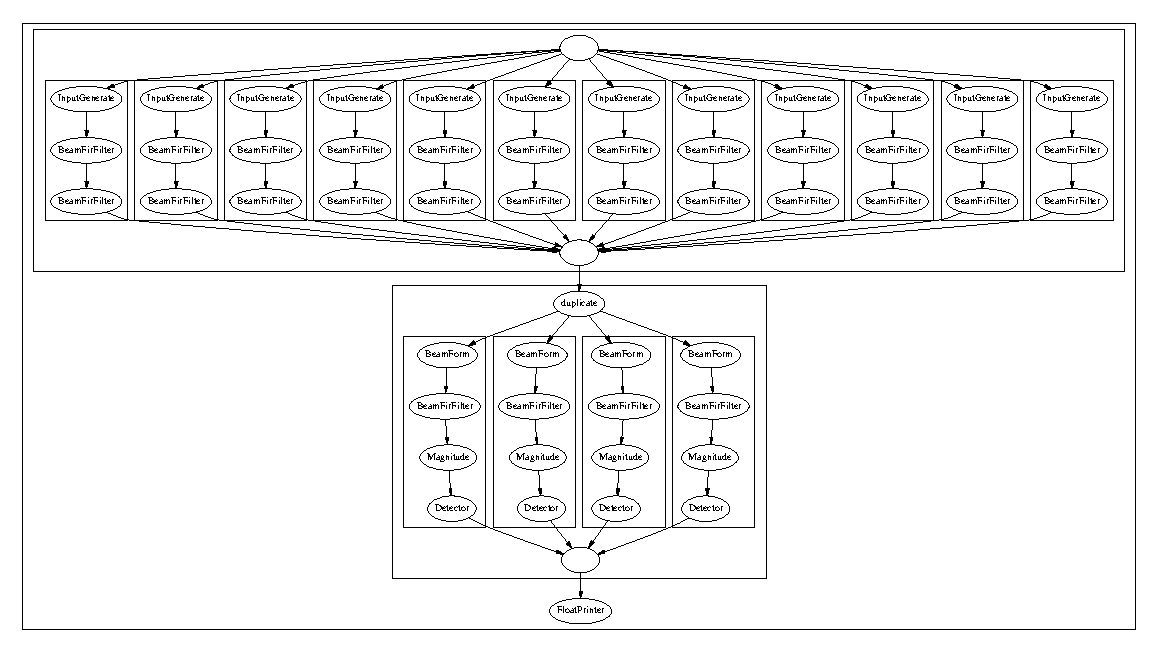
\includegraphics[width=6.0in]{figures/beamformer.eps}
  \caption{A DSP block diagram of the application Beamformer}
  \label{fig:block-diagram}
\end{figure}

    Blocks can be characterized in various ways. The simplest characterization
of blocks is a \textit{linear} block, defined as a module that
outputs a linear combination of its inputs plus a constant term. A
linear block can be represented by a matrix relating inputs to
outputs and a vector of constants. The next simplest
characterization of blocks is \textit{linear state-space}. Such a
block uses a set of state variables. The output of this block is a
linear combination of its inputs and state variables. In addition,
the state variables are updated by a linear combination of
themselves and inputs.  A linear state-space block can be
represented by four independent matrices.

    A linear state-space characterization is more general than a
linear characterization - all linear blocks are also linear
state-space blocks, but the converse is not true. The intuitive
reason for this fact is that a linear block is memoryless, meaning
the outputs only depend on current inputs. However, a linear
state-space block has memory in the form of state variables, so
the outputs depend on current inputs and past inputs.

    We will perform analysis and optimization of DSP applications at
the linear state-space level. We choose this representation
because it models a wide class of applications or parts of
applications, and it is simple to work with.

    Our work with state-space representations will be done in the
context of StreamIt, a programming language designed for streaming
applications \cite{streamitcc}.  StreamIt allows users to create
their own blocks, but limits the way these blocks can be
connected. We perform the following steps on a StreamIt program:

\begin{enumerate}
\item Examine each block and determine whether or not it can be
characterized as linear state-space. If it can, extract the
appropriate state-space representation.

\item Combine connected blocks that each have a state-space
representation, using an appropriate set of rules depending on the
type of connection.

\item Optimize representations through the use of state-space
transformations.

\item Convert the state-space representation(s) back to StreamIt
code.
\end{enumerate}

\section{Organization}

    The rest of this thesis is organized as follows.  In Chapter 2 we
provide background information about StreamIt and formal linear
and linear state-space models.  Chapter 3 is devoted to
state-space analysis of StreamIt programs (Items 1, 2, and 4).
Chapter 4 describes optimizations (Item 3). In Chapter 5 we
discuss our implementation and results.  Chapter 6 details related
work.  In Chapter 7 we provide our conclusions and list possible
future work.

\chapter{Background and Related Work}\label{ch:bg}

Streaming languages provide an attractive alternative to sequential languages for many applications. In a streaming language, the programmer defines actors that operate on data streams and composes programs by connecting actors. Many common high-performance applications, especially those involving signal, audio, image, and video processing, have explicit block diagram structure and are most easily conceptualized in that manner, making streaming languages a natural choice for these applications.

Because programs written in streaming languages are explicitly structured as communicating actors, they typically expose a high degree of parallelism. This allows streaming language compilers to easily analyze stream programs and efficiently parallelize them. Compared to sequential languages, streaming languages free the programmer from the burden of having to explicitly write parallelized code for specific architectures, allowing him to focus on expressing the high-level semantics of the algorithm in a natural way.

Recent developments in streaming languages include Brook~\cite{brook}, Cg~\cite{cg}, and StreamC/KernelC~\cite{streamc}.

\section{The StreamIt Programming Language}\label{ch:bg:str}

StreamIt~\cite{asplos02} is a high-performance streaming language developed at MIT. StreamIt is based on the Synchronous Dataflow model of streaming computation. In the SDF model~\cite{sdf}, actors are constrained to known, fixed communication rates. This restriction makes it easier for compilers to analyze the stream graph and schedule actors for efficient parallel execution. StreamIt further extends the SDF model with additional language elements that impose hierarchical structure on the stream graph and provide additional expressive power. The StreamIt language also places a high degree of emphasis on code reuse. All of these features serve to increase programmer productivity; complex applications have been written in StreamIt, including an MPEG2 encoder and decoder~\cite{mpeg} and image-based motion estimation~\cite{basier}.

The structure and parallelism exposed by StreamIt programs allows the StreamIt compiler to perform a large set of optimizations and efficiently execute programs on parallel architectures. The compiler targets a number of architectures, including standard unicore and multicore processors, computing clusters, and the Raw processor.\footnote{A Cell backend is currently under development; the work done in this thesis directly contributes to that.}

\subsection{Filters}

The basic unit of a StreamIt program is the \emph{filter}. This construct represents an actor that reads data items from a single input tape, processes them, and writes data items to a single output tape. Filters are allowed to \emph{pop} items from the input tape, \emph{push} items onto the output tape, and \emph{peek} at items on the input tape without removing them. Individual filters are independent and communicate only through the data items on their tapes. Each filter must define a \emph{work function} that specifies the work done by each iteration of the actor; work functions are written in a general-purpose sequential language that resembles Java in syntax. Work functions are required to be annotated with pop, peek, and push rates, which (for the purposes of this thesis) must be static and fully known at compile time.

Filters can also define constants and arbitrary helper functions. In addition, filters may declare mutable fields; this creates \emph{state} that is maintained across work function iterations. Filters can be declared with parameters that are provided when filters are instantiated, creating significant opportunities for code reuse.

\subsection{Composing Streams: Pipelines and Splitjoins}

StreamIt provides the \emph{pipeline} and \emph{splitjoin} constructs to compose StreamIt constructs in a hierarchical manner. Each StreamIt construct has a single input tape and single output tape, allowing for arbitrarily deep hierarchical composition.

The \emph{pipeline} construct connects multiple child streams (which may be filters, pipelines, or splitjoins) in a pipeline, with the input tape of each stream connected to the output tape of the previous stream in the pipeline.

The \emph{splitjoin} construct splits a stream into multiple child tasks. At the top of a splitjoin, a \emph{splitter} splits the single input tape into multiple tapes. StreamIt allows two types of splitters: \emph{duplicate} splitters, which copy every item on the input tape to every output tape, and \emph{round-robin} splitters, which send each item on the input tape to a different output tape in weighted round-robin fashion. The child streams of the splitjoin have their input tapes connected to the outputs of the splitter. At the bottom of the splitjoin, a \emph{joiner} joins the outputs of the child streams into a single output tape. Joiners always operate in weighted round-robin fashion.

\subsection{Execution Model and Compiler Optimizations}\label{ch:bg:str:exec}

A full StreamIt program consists of a top-level stream (a filter, pipeline, or splitjoin) that defines a hierarchical stream graph. At the leaves of the hierarchy are individual filters, connected by channels. When a StreamIt program executes, the top-level stream is implicitly wrapped in an infinite loop.

A \emph{steady state} is a repetition of each filter such that when the steady state is executed, the amount of data in all channels remains unchanged. The StreamIt compiler performs optimizations and execution in terms of the steady state.

The stream graph of a StreamIt program exposes three types of coarse-grained parallelism:
\begin{itemize}
\item Task parallelism: parallelism explicitly defined by the stream graph. For instance, the child streams of a splitjoin are task-parallel; they have no dependencies on each other, and can be run in parallel.
\item Data parallelism. Filters that are stateless are data-parallel; different iterations of a data-parallel filter have no dependencies on each other, and thus multiple instances of a data-parallel filter can be simultaneously run to process data from different iterations of the stream graph.
\item Pipeline parallelism: parallelism exposed by filters connected in a pipeline.
\end{itemize}

Pipeline parallelism can be exploited by using coarse-grained software pipelining.~\cite{asplos06} An initialization schedule is first run to set up sufficient data in all channels. Thereafter, whenever the steady state schedule is run, there are no longer any dependencies between different filters in the steady state, allowing multiple filters to be executed in parallel.

The StreamIt compiler uses all three types of parallelism to achieve optimal performance on parallel architectures. The compiler can also \emph{fuse} multiple filters together, producing a single filter. This fused filter typically has a lower communication--computation ratio than the original filters. When stateless filters that do not perform peeking are fused, the result is also a stateless (and hence data-parallel) filter that does not peek.

\subsection{Extensions}

The full StreamIt language provides a number of additional features beyond the basic model described above. In particular, StreamIt supports \emph{i}) an additional \emph{feedbackloop} construct, which defines a feedback loop that introduces a cycle into the stream graph, \emph{ii}) filters with dynamic rates that need not be fixed or known at compile time, and \emph{iii}) teleport messaging for out-of-band communication between filters~\cite{messaging}. These language features greatly increase the power of language, allowing more complex applications to be more easily written.

The StreamIt compiler is also able to perform cache-aware~\cite{cacheopt} and domain-specific~\cite{linear03,linear05} optimizations.

\section{The Cell Architecture}\label{ch:bg:cell}

The Cell architecture~\cite{cell:website,cell:intro,cell:arch,cell:handbook} is a novel multicore architecture designed for high-performance computing. Compared to a standard SMP architecture, Cell has two major differences:
\begin{itemize}
\item Cell is a heterogeneous architecture consisting of nine cores per physical processor. One core, the Power Processing Element (PPE), is a general-purpose processor. The other eight cores are Synergistic Processing Elements (SPEs) that are dedicated for computation.
\item Cell is not a shared-memory architecture. SPEs can only directly address their own limited local store. Programmers have explicit control over DMA operations to copy data between local store and memory.
\end{itemize}

\subsection{PPE}

The PPE is a 64-bit, two-way SMT, PowerPC-compatible processor.\footnote{The word size on Cell is considered to be 32 bits. A common unit of data is the quadword, which is 16 bytes.} All system code is run on the PPE. The PPE also contains additional facilities for supporting and controlling SPEs.

The PPE is designed as a control processor, and is not optimized for computation. It has a simplified in-order pipeline with no dynamic branch prediction. In addition, many instructions on the PPE (such as integer multiply and divide) are not pipelined.

\subsection{SPEs}

SPEs are designed to act as dedicated computation units. Each SPE has a large 128-entry register file; all registers are 128-bit SIMD registers that can be treated as short vectors of any of the standard integer or floating point data types. Each register can also be treated as the scalar value that occupies the first element of the vector. SPEs have a separate instruction set from the PPE; all computation instructions are SIMD and operate on all elements of a register, with different forms provided for each supported data type. However, SPEs are optimized for single-precision floating-point operations.

SPEs also have a simplified in-order pipeline without dynamic branch prediction. The SPE pipeline supports dual-issue of certain pairs of instructions. In general, the design of the SPE moves the task of instruction scheduling from the processor to the compiler or programmer.

Each SPE has its own 256 KB local store (LS).\footnote{We will sometimes use the term \emph{SPE} to refer to the SPE's local store, and \emph{PPE} to refer to memory; the usage should be clear from the context.} SPE load and store instructions can only directly access local store; all code and data that an SPE uses must be located in its local store. Loads and stores can only be done on a 16-byte granularity; loading a scalar that is not aligned on a quadword boundary requires an additional rotate instruction, and storing a scalar requires a read-modify-write operation. SPEs have no cache; however, loads and stores have short 5-cycle latencies and are fully pipelined (in effect, the local store acts as a software-controlled cache).

SPEs do not have paging or protection facilities, and all code running on an SPE is application code. In order to read or write data in memory, SPE programs must explicitly use special instructions to initiate DMA operations. Each SPE contains a Memory Flow Controller (MFC) that handles DMA transfers; once an SPE program has started a transfer, the MFC carries it out in the background while the SPE continues to execute and access local store. The SPE can poll or elect to receive interrupts when DMA operations complete. The MFC supports up to 16 concurrent DMA transfers.

The MFC uses the page tables on the PPE to perform address translation; thus, SPEs can access the entire virtual address space of the program through DMA. Each SPE's local store, as well as special communication channels, is mapped into the virtual address space; the PPE can access an SPE's local store directly and other SPEs can access its local store or communication channels through DMA.

SPEs provide two facilities for communicating small messages with the PPE and other SPEs: mailboxes and signal notification registers. They are mapped into the program's virtual address space as MMIO registers, and other processors (either the PPE or other SPEs) can access them through the corresponding memory addresses. Mailboxes are 32-bit FIFOs. Each SPE provides an inbound mailbox with 4 entries for receiving messages from other processors, an outbound mailbox (1 entry) for sending messages to other processors, and an outbound mailbox (1 entry) for sending messages to the PPE (messages written to this mailbox generate interrupts on the PPE).

Each SPE provides two 32-bit signal notification registers that other processors can write to. Each bit in a signal notification register ``latches'' the highest bit received until the register is read by the SPE. SPEs can poll for mailbox messages and signals, or elect to receive interrupts.

\subsection{DMA}

The PPE and SPEs are connected to each other and to memory by a high-bandwidth communication bus. The startup cost of a typical DMA operation is around 100 to 150 ns;~\cite{cell:micro} afterwards, 8 bytes can be transferred per SPE cycle. The communication bus provides extremely high bandwidth: each processor has access to 25.6 GB/s of bandwidth, and the bus can theoretically support a peak bandwidth of over 200 GB/s.

DMA transfers have specific alignment requirements: transfers must be 1, 2, 4, 8, 16, or a multiple of 16 bytes, up to 16 KB. Transfers less than a quadword must be between memory and LS addresses that are naturally aligned;\footnote{That is, aligned on a multiple of the transfer size.} larger transfers require addresses that are quadword-aligned. DMA transfers are most efficient when memory and LS addresses have the same offset in a 128-byte block; the author experimentally determined that transfers that do not effectively have only half the maximum bandwidth.

\subsection{Performance and Programmability}

IBM provides an SDK that contains separate C/C++ compilers to target the PPE and SPEs. C intrinsics are provided to access the unique facilities defined on the Cell processor.

The initial version of the Cell processor has a clock speed of 3.2 GHz. The SPE instruction set contains a fully pipelined SIMD single-precision floating-point multiply-add instruction, which performs 8 FLOP in a single cycle. Thus, a single SPE is theoretically capable of 25.6 GFLOPS; the entire Cell processor is capable of 204.8 GFLOPS using only the eight SPEs. A standard general-purpose processor with a SIMD unit, running at the same clock speed, has the same theoretical maximum performance as only a single SPE.

Achieving good performance on Cell requires a number of considerations. It is important to make heavy use of SIMD instructions and carefully schedule instructions to maximize utilization of the SPE pipeline. For instance, a sample single-threaded application\footnote{This is the FFT benchmark, described more fully in chapter~\ref{ch:use}.} that operates on scalar data, when compiled for different processors using GCC with standard compiler optimizations (\textsf{-O3}; no vectorization was performed), produces runtimes given in figure~\ref{fig:cell:proc} (SPE time does not include communication).

\begin{figure}[!htb]
\begin{center}
\begin{tabular}{|r|r|}
\hline
& Runtime (ms) \\
\hline
PPE, 3.2 GHz & 220 \\
\hline
1 SPE, 3.2 GHz & 400 \\
\hline
Pentium 4, 1.8 GHz & 200 \\
\hline
Xeon, 2.2 GHz & 170 \\
\hline
\end{tabular}
\end{center}
\caption{Runtimes for FFT on different processors.}
\label{fig:cell:proc}
\end{figure}

Compared to the PPE, the better performance of the Intel processors, which have significantly lower clock speeds, can be attributed to the latter's incorporation of out-of-order and superscalar execution logic. The significantly worse performance of the SPE is due to the additional rotate instructions necessary to operate on scalar data. Compared to general-purpose architectures that have complex out-of-order, superscalar pipelines, the Cell architecture requires more work from the compiler or programmer to generate code that executes efficiently.

Obviously, performance on any parallel architecture requires being able to discover and execute multiple parallel tasks in an application. On Cell, the data used by individual tasks that execute on SPEs must be sized for the limited local store, and their memory access patterns must be tuned for coarse-grained bulk DMA transfers, potentially requiring reorganizing the program or reorganizing data layout. While frameworks exist that provide software-managed caches for SPEs,~\cite{cell:website} it is ultimately simpler and more efficient if memory access patterns by SPE programs can be kept as local as possible.

Finally, it is important to leverage the communication--computation concurrency provided by Cell's asynchronous DMA model by performing computation while data for future work is being fetched. If double-buffering is done properly, SPEs will be able to spend a majority of their time performing useful computation.

All three of the issues above must be carefully considered for an application to obtain maximum performance from the Cell architecture. Some applications, such as matrix multiplication, can be aggressively optimized for Cell to achieve close to peak performance.~\cite{cell:intro}

\section{Parallelization Frameworks}

MPI and OpenMP are probably the two most well-known and widely used parallelization frameworks for computing clusters and traditional SMP architectures. These two programming APIs represent opposite ends of a spectrum: MPI defines a language-independent, low-level network communication API, while OpenMP defines a set of language-specific, high-level annotations that programs can use to cause compatible compilers to generate multithreaded code.

The streaming runtime library for Cell developed in this thesis is intended to provide the same kind of low-level functionality as MPI, with two major differences: \emph{i}) it is specific to Cell instead of networks, and \emph{ii}) it is specific to streaming applications and provides additional control functionality.

Several languages and parallelization frameworks have been designed specifically for Cell; see \cite{cell:pf} for a review. RapidMind~\cite{rapidmind}, MPI Microtask~\cite{mpimicrotask}, and Sequoia~\cite{sequoia} follow a ``task-based'' approach by providing runtime systems that help schedule program-defined tasks, or kernels. CellSs~\cite{cellss} takes this a degree further by automatically generating tasks from annotations to linear code.

\section{The Streaming Runtime Library for Cell}\label{ch:lib}

The Cell architecture provides an excellent target for streaming language compilers for a number of reasons:
\begin{itemize}
\item Individual SPEs are optimized for computation.
\item The limited local store available on SPEs is not a severe limitation for actors in a stream program, which are independent, have extremely local data-access patterns, and generally have small code sizes. In an SDF model such as the basic StreamIt model, known static rates further simplify scheduling.
\item The high-bandwidth, low-latency on-chip communication network enables a large number of scheduling options which would not be feasible for other targets, such as computing clusters.
\end{itemize}

The natural division of work on the Cell architecture maps computation to SPEs, which perform DMA operations to copy input and output data to/from local store. In this model, the PPE functions mainly as a control processor, possibly also performing small amounts of computation that are too small to dispatch to an SPE.

Using this model, a streaming language compiler (or programmer) must address four major issues:
\begin{enumerate}
\item Generating highly-SIMDized code in the limited SPE instruction set. SIMD is required to make full use of an SPE's execution units. In addition, code that operates only on vectors avoids rotate instructions needed to load scalar values from local store, in effect producing a greater performance improvement than would be expected.
\item Generating code that performs DMA operations. This code also needs to double-buffer input and output to make full use of Cell's asynchronous communication model.
\item Organizing all needed code and sufficient buffering to fit into limited SPE local store. This is particularly a problem for larger applications, for which the total code size for all filters leaves little room for buffering, or may exceed the size of local store entirely.
\item Performing high-level optimizations and scheduling. At a high level, compilers would typically be interested in balancing workload among available SPEs, avoiding excess communication, transforming code to improve efficiency, and other such topics.
\end{enumerate}

The purpose of the streaming runtime library for Cell is to abstract \textsf{(2)} and provide facilities that simplify \textsf{(3)} and \textsf{(4)}. The library frees a compiler or programmer from needing to deal with the details of Cell's communication model, allowing it to focus on exploring high-level optimization and scheduling choices. The two main functions of the library are:
\begin{itemize}
\item Providing high-level facilities in place of explicit DMA operations between SPE local stores and memory.
\item Providing the \emph{user}\footnote{\emph{User} refers to all non-library code running on the PPE; typically, most of this performs scheduling. Code for filter work functions and auxiliary functions will always be referred to separately.} with a generic framework for controlling and dispatching computation to SPEs that simplifies scheduling operations.
\end{itemize}

While the library was designed with StreamIt constructs in mind, it is not specific to that language. The library can be used with filters and stream graphs that follow a basic set of specifications, regardless of the original streaming language.

\section{Library Constructs}

The library defines several constructs for the SPEs and PPE. Most facilities provided by the library operate on one or more of these constructs.

\subsection{SPE Constructs: Filters and Buffers}

Two basic constructs are defined for SPEs: \emph{filters} and \emph{buffers}.

\emph{Filters} have similar semantics as StreamIt filters, but are more generalized. A filter represents a generic actor that exposes a work function which is conceptually run infinitely. Filters may be stateful and can read from multiple input tapes and write to multiple output tapes. While a library filter can correspond directly to a single filter in a StreamIt program, a compiler can also perform optimizations, such as fusing multiple StreamIt filters into a single library filter. Work functions are opaque to the library and the library does not perform any SIMDization; that task is left to the compiler or programmer.

\emph{Buffers} are contiguous regions of SPE local store that are reserved for temporarily storing data that is on an input or output tape. All buffers are circular, and the library maintains head and tail pointers for each buffer that indicate where data begins and ends. Conceptually, a buffer has front and back ends; data towards the front of a buffer originated earlier in the execution of the program.

Conceptually, a filter consists of two major components, \emph{code} and \emph{state}, as well as basic properties that describe its work function such as the number of input and output tapes. \emph{Code} is a single contiguous block of arbitrary data that may contain constant data and instructions that define multiple functions; the library only requires that it contain a function with a specific signature, which is used as the work function. Code for a filter is intended to be a single modular component that can be easily relocated to different local store addresses on different SPEs. As such, it should not reference any absolute addresses, such as in absolute branches or loads, or modify itself.\footnote{If the user can accept limitations, such as not being able to relocate filter code or tying code to a single SPE, these suggestions can be ignored.} The latter constraint means that code should not contain any global variables; instead, all global variables should be declared and accessed through fields in the filter's state. \emph{State} contains all mutable data that must be maintained across iterations of the work function. State for different filters is disjoint, and filter code should not access mutable global state. Although a filter's code and state must reside in SPE local store when the filter's work function is running, every filter must have a permanent store for them in memory. The library provides facilities for loading code onto SPEs and copying state between local store and memory.

A filter's work function typically accesses its tapes by reading from the front of its input buffers and writing to the back of its output buffers. This is not enforced by the library and filters can have other data access patterns; however, the library is designed to expect this pattern and the user must take special care otherwise. Filter work functions do not need to have static rates, and the library is agnostic to a filter's rates.

Before a filter can be run on an SPE, it must be loaded onto the SPE through the library. The user provides the library with the properties of the filter and the LS address of its work function; the library initializes a control block that describes the loaded filter in local store, the LS address of which identifies the loaded filter in all future operations. If the filter is stateful, the library also copies its state into local store from its permanent store in memory. Code for the filter must be separately copied into local store through the library, but can be located anywhere as long as the correct work function address is provided to the library. When the user is done with a loaded filter, it can unload the filter through the library, causing the library to copy the filter's state back to its permanent store in memory. Stateful filters can be loaded on at most one SPE at any time, while stateless filters can be simultaneously loaded on any number of SPEs.

This separation of code and state allows the user additional control over how and when SPE local store is used. Since code is constant, the user can preload the code of a filter onto an SPE even while the filter is loaded on another SPE (and thus its state is owned by that SPE) in preparation for loading it on the first SPE in the future. If multiple (possibly stateful) filters have identical code, only one copy of it needs to reside in memory or an SPE's local store and it can be shared. When a filter is not being run, its code does not need to be present in SPE local store, leaving more space free for buffering (local store management is discussed in more detail below).

The library provides similar facilities for allocating buffers on SPEs. The size of a buffer must be a power of two, to allow wrap-around computations to be done with a single \textsf{AND} instruction. Buffers are identified by the LS address that their data region starts at in SPE local store; when allocating a buffer, the library initializes a control block located immediately before the data region that stores the buffer's head and tail pointers and participates in data transfers. As an additional step required before a loaded filter can be run, the user must specify which buffers the filter's input and output tapes refer to.

The library does not provide memory management for SPE local store; when filter code, filter control blocks, and buffers are allocated, the user must manually specify their LS addresses and ensure that the regions used by different constructs do not overlap.\footnote{The library handles all resulting communication, such as copying filter code and state.} This does not create as many difficulties as may appear, as any memory management algorithm that can be implemented internally by the library can just as easily be duplicated by the user on the PPE. Moreover, allowing the user to explicitly manage local store allows it to implement far more complex algorithms as desired. Additionally, in this scheme, buffers and space occupied by filter code and filter control blocks for stateless filters never need to be explicitly deallocated -- the user can simply reuse the local store region for other constructs after it is certain that they are no longer in use.

Theoretically, the number of filters loaded and buffers allocated on an SPE is limited only by available local store. However, there is generally no useful purpose in keeping more than two filters and their associated buffers on an SPE at any time.

\subsection{PPE Constructs}

The library does not define a filter construct for the PPE. However, because all memory is addressable by PPE code, the user can easily create similar behavior.

The library defines a PPE or memory buffer construct that is an extension of the SPE buffer. PPE buffers are not required to be circular, and buffers that are non-circular have no size limitations. PPE buffers are identified by the address of their control block, and multiple buffers can refer to the same data region, with different head and tail pointers. This is used to implement certain StreamIt features with minimal overhead, such as duplicate splitters and data-parallel execution. Because of the limited size of SPE local store, this functionality was considered unnecessary for SPE buffers.

Conceptually, data produced during the execution of a program is contained in exactly one buffer (which may be an SPE or PPE buffer) until it is consumed. The library provides facilities for moving data between buffers on different processors.
 
\section{Library Commands}

Under the library, SPEs only execute library code and filter code. User code on the PPE dispatches work items to SPEs by issuing library \emph{commands}, and is notified when SPEs complete them. Each library command encapsulates a specific action to be performed, and has parameters that are specified by the user. Commands can be divided into three main types:
\begin{itemize}
\item Filter commands: commands to load or unload filters, copy filter code into local store, attach tapes to buffers, and run filters.
\item Buffer commands: commands to allocate buffers.
\item Data transfer commands: commands to move data between buffers in the local stores of different SPEs, or local store and memory.
\end{itemize}

As an example, the \textsf{filter\_run} command, which runs a loaded filter, takes two parameters: the LS address of a loaded filter's control block, and the number of iterations to run the work function for. The user is responsible for ensuring that there is sufficient data in input buffers and sufficient space in output buffers for all specified iterations. Other commands have similar requirements. For a complete description of all commands, see appendix~\ref{app:ui:cmd}.

The amount of work specified by a single command varies depending on parameters to the command. Typically, \textsf{filter\_run} commands do not take more than a few hundred microseconds to complete; some other commands are auxiliary commands and complete almost immediately. This allows the user to quickly change scheduling decisions and avoids tying an SPE into any specific long-term action.

When the user issues a command to an SPE, it assigns the command an ID that must be unique among all commands previously issued to that SPE that have not completed. This ID is used to notify the user when the SPE finishes executing the command. 

\subsection{Dependencies}

In order to keep SPEs supplied with work at all times, it is necessary to limit round-trips between the PPE and SPEs during which the SPEs have no commands to execute. The library provides a general facility for queuing and ordering commands on individual SPEs by allowing each command to specify a set of command IDs on that SPE that it depends on. Commands issued to an SPE are queued and executed only after all dependencies have finished.

At any time, a command that has been issued to an SPE can be either \emph{queued} (a command with unfinished dependencies), \emph{active} (a command with all dependencies satisfied and currently being executed), or \emph{completed} (a command for which all work has been done, but the user has not yet been notified). From the perspective of the user, all commands that are active on an SPE are run ``concurrently''. When a command is issued, all dependency IDs that have not been issued are considered to have already completed and are ignored.

In effect, each SPE maintains a small dependency graph of commands that represents a small subset in time and space of the entire schedule the user executes a program with. User code on the PPE continually adds commands to the dependency graph, while the SPE continually processes commands that have their dependencies satisfied. To make full use of an SPE, it is only necessary for the PPE to ensure the dependency graph on the SPE is never empty. The user cannot remove commands once issued, but if it keeps the dependency graph low-depth, it can quickly change the pattern of work done by an SPE simply by issuing a different set of new commands.

\subsection{Command Groups}

Each command has a small amount of data associated with it, consisting of command-specific parameters in addition to generic ID and dependency information. Typically, the user will be issuing sets of related commands at once. To avoid the overhead of issuing each command individually, the user can organize commands into groups; the library only allows entire command groups to be issued.\footnote{To issue a single command, the user can create a group containing only that command.} Each group specifies a sequence of commands; until a group is explicitly cleared, commands in the group are saved and can be reissued in the future.

Since SPE local store is managed by the user, the user must provide the library with an LS address where command data will be copied to when it issues a command group. For dependency purposes, SPEs treat commands in a group as having been issued in the order they appear in the group. Although commands are issued in groups, the user is notified when individual commands complete.

\subsection{User Interface}

Commands issued to different SPEs are completely independent; the dependency graph on each SPE is strictly local. User code on the PPE thus serves as the main point of synchronization between SPEs by adjusting the commands it issues to an SPE in response to command completion notifications from all SPEs.

User code on the PPE is mainly callback-driven. The user registers a callback function with the library that is called whenever a command issued to an SPE completes. The library maintains a per-SPE bitmap of command IDs that have completed; the user can query this bitmap in the callback to determine which commands have completed and respond accordingly. Bits in the bitmap are set until explicitly acknowledged by the user. After an ID has been acknowledged, it can be reused for new command issued to the SPE.

The library does not maintain a dependency graph on the PPE. Some SPE commands have equivalents on the PPE provided as library functions, which are run immediately when called.

Appendix~\ref{app:ui} contains complete specifications for the interface provided by the library to user code.

\subsection{Data Transfer}

Data transfer commands indirectly result in additional points of synchronization between processors. A data transfer conceptually moves data from the front of a source buffer to the back of a destination buffer, and requires two commands: a command to transfer data out of the source buffer, issued to the processor containing the source buffer, and a command to transfer data into the destination buffer, issued to the processor containing the destination buffer. Where either buffer is located in memory, the user instead calls a library function.

Splitting data transfers into a pair of commands with one on each processor provides the user with explicit control over when the data transfer occurs with respect to both processors. The library ensures that the transfer does not occur until both commands become active on their respective processors. The user must ensure, via the dependency graphs on SPEs or manually on the PPE, that when a data transfer command becomes active on a processor, the local buffer has sufficient data or space to fulfill the transfer.

Data transfers impose minor alignment requirements on the buffers involved due to limitations of Cell's underlying DMA model. There are no restrictions on the size of a data transfer (except for the size of the buffers involved), but the same size must be specified by both commands in the pair. Each data transfer command also specifies the address and size of the opposing buffer, since this is information the user will know in advance; however, buffer head and tail pointers, which are more difficult to track in advance, are handled by the library. In addition, data transfer commands have additional inter-SPE requirements that the user must ensure are met across all SPEs. When a data transfer command becomes active on an SPE, the opposing buffer must already be allocated on the opposing SPE. As well, for any buffer, at most one data transfer in command and one data transfer out command specifying it as the opposing buffer can be active at any time across all processors.

This ``decoupling'' of data transfers simplifies the information the user needs to keep track of. When issuing commands to one SPE, the user usually does not need to be concerned with the state of other SPEs; as long as pairs of data transfer commands are eventually issued with the correct parameters and dependencies, the library will handle synchronization between buffers.

\section{Filter Code}

The interface provided by the library for writing filter code consists of a set of C header files that define a collection of preprocessor macros that simplify state and tape access. StreamIt code can be converted almost directly to code for a library filter. For complete specifications, see appendix~\ref{app:filterui}.

\section{User Code Examples}

As an example, we will illustrate the commands required to set up and run a sample filter on an SPE. For simplicity, this filter has a single input tape, single output tape, and static rates: its work function pops $i$, peeks $i+e$, and pushes $o$ bytes per iteration.

Before the filter can be run, it must be loaded, its input and output buffers must allocated, and the filter's tapes must be attached to the buffers. The commands that perform this are illustrated in figure~\ref{fig:lib:init}.

\begin{figure}[!htb]
\begin{center}
\includegraphics{figs/init}
\end{center}
\caption[Commands to set up a filter.]{Commands to load a filter and allocate and attach input and output buffers. Lines between commands represent dependencies that must be specified to the library when the commands are issued. These commands may be issued in one or multiple groups. See appendix~\ref{app:ui} for detailed information on setting up commands and dependencies.}
\label{fig:lib:init}
\end{figure}

In addition, input data must be transferred into the input buffer before the filter can be run, and output data must eventually be transferred out of the output buffer. With an initially empty input buffer, the commands to transfer in $n$ iterations of input, run the filter for $n$ iterations, and then transfer out $n$ iterations of output (assuming that the input and output buffers were sized appropriately) are shown in figure~\ref{fig:lib:run}.

\begin{figure}[!htb]
\begin{center}
\includegraphics{figs/run}
\end{center}
\caption[Commands to run a filter.]{Commands to run a filter for the first $n$ iterations, including transferring input and output. The corresponding data transfer commands on other SPEs or the PPE are not shown.}
\label{fig:lib:run}
\end{figure}

To run the filter for a larger number of iterations, a sequence of commands is required due to the limited buffer space available in SPE local store. This is illustrated in figure~\ref{fig:lib:ext}.

\begin{figure}[!htb]
\begin{center}
\includegraphics{figs/ext}
\end{center}
\caption[Sequence of commands to run a filter for a large number of iterations.]{Sequence of commands to run a filter for a large number of iterations. Command IDs are indicated in the upper right. Each row is issued as a different group.}
\label{fig:lib:ext}
\end{figure}

Provided that the input buffer is at least $2ni+e$ bytes and the output buffer is at least $2no$ bytes, the dependencies among the commands in the sequence ensure that:
\begin{itemize}
\item When a \textsf{dt\_in} command becomes active, there are at most $ni+e$ bytes of data in the input buffer, and thus enough space to transfer in an additional $ni$ bytes.
\item When a \textsf{dt\_out} command becomes active, there are at least $no$ bytes of data in the output buffer, and thus enough data to transfer out.
\item When a \textsf{filter\_run} command becomes active, there are at least $ni+e$ bytes of data in the input buffer and at most $no$ bytes of data in the output buffer. This is enough input data and output space to run the filter for $n$ iterations.
\end{itemize}

This sequence of commands effectively ``pipelines'' the basic operation from figure~\ref{fig:lib:run}. Double-buffering is accomplished when the data transfer commands in a group complete before the \textsf{filter\_run} does. In this case, the following \textsf{filter\_run} has no outstanding dependencies once the current \textsf{filter\_run} completes, and can become active immediately.

The user can keep the SPE continually supplied with work by initially issuing the first two groups, thereafter issuing the next group whenever a group completes. In this case, the SPE almost always has two groups of commands issued, with one group active and the other queued. In addition, with the exception of the first two and last two groups, the command parameters, IDs and dependencies in every other group are identical. This allows the user to initially set up two groups ($g_0$ and $g_1$ in figure~\ref{fig:lib:ext}) and repeatedly issue them for a majority of the execution. If executions are relatively long, the overhead of the first and last group, where no filter is being run, will be amortized effectively. Alternatively, the user can load another filter and run it during those gaps.

In practice, situations such as the above, where a static-rate filter is run for a large number of iterations and large amounts of input and output data are transferred, are very common. To avoid requiring the user to manually issue groups and deal with command completion callbacks in every such case, the library also provides extended operations that encapsulate this pattern. In an extended operation, the user provides the library with filter rates, the addresses of opposing buffers on other processors for data transfers, and the number of groups to run for; the library issues and responds to all commands internally and notifies the user when the entire operation is complete. Where one or both opposing buffers are located in memory, the library also handles the PPE side of data transfers internally. Extended operations greatly simplify setting up pipelines of any length where all filters in the pipeline have static rates.

\section{Library Implementation}

The library is implemented as three separate components: \emph{i}) runtime code for SPEs, \emph{ii}) basic runtime code for the PPE, and \emph{iii}) runtime code for the PPE that handles extended operations.

\subsection{PPE Implementation}

For each SPE, the library maintains a fixed table of command groups in memory. Each entry in the table represents a group and stores command data for commands in the group. When the user issues a group to an SPE, the library sends a mailbox message to the SPE to notify it of the entry in the table that contains the group and the LS address to copy command data to; the use of a fixed table is directly necessary to be able to pack all required fields into a single 32-bit mailbox message. After receiving the mailbox message, library code on the SPE initiates DMA to copy command data into local store.

When commands are completed by an SPE, library code on the SPE sends a bitmap of the command ID(s) to the PPE via the outbound mailbox. If the mailbox is full (the PPE has not had time to respond to the previous message), the bitmap is queued and sent when the mailbox is empty. The size of a mailbox message (32 bits) currently imposes a strict limit on the range of valid command IDs.

Library code on the PPE continually polls the outbound mailboxes of all SPEs in round-robin order for command completion messages. When a message is received, it is processed by the library, which eventually runs the user-registered callback. Interrupts were not used as each interrupt requires approximately 7 $\mu$s of kernel time to process. Although this may be negligible when only a single SPE is involved, it can become significant when multiple SPEs are all generating interrupts. In general, it is the author's opinion that the Cell architecture's focus on directly using SPEs to run small pieces of application code is not suited for the additional system overhead of interrupts.

One major drawback of the continuous polling approach is that it severely constrains any other work that the PPE is able to perform unless the user is willing to call the library function that performs polling at regular intervals. This is not a problem when the PPE is used solely as a control processor; most control computations are in response to command completion messages from SPEs and can be done in the callback.

The sequence of events that occurs on the PPE and an SPE between the time the user issues a group of commands and the user being notified of the completion of a command in the group via callback is illustrated in figure~\ref{fig:lib:control}. In actuality, because \emph{i}) each SPE is issued multiple commands and \emph{ii}) the PPE is controlling multiple SPEs, there will typically be many different copies of this sequence interleaved within each other, for both the same and different SPEs.

\begin{figure}[!htb]
\begin{center}
\begin{tabular}{rp{2.5in}p{2.5in}}
& \emph{PPE} & \emph{SPE} \\
\cline{2-3}
& Continually polls for command completion messages from SPEs. & Continually polls for mailbox messages while running active commands. \\
\cline{2-3}
\textsf{(1)} & \emph{User creates new group and adds commands.} Command data is written to entry in groups table. & \\
& \emph{User issues group.} Sends mailbox message to SPE. & \\
& & Receives and unpacks mailbox message. Copies command data (using DMA) from table entry to local store at specified LS address. \\
& & After copying command data, adds new commands to dependency graph. \\
& & \multicolumn{1}{c}{$\cdots$} \\
& & When command(s) complete, writes bitmap of completed ID(s) to PPE. \\
& Receives command completion message and calls user-defined callback. & \\
& \emph{Inside callback, user sets up and issues new groups if desired.} Repeats from \textsf{(1)}. &
\end{tabular}
\end{center}
\caption[SPE control protocol.]{SPE control protocol. \emph{Italicized} text represents actions performed by user code. All other actions are performed by library code.}
\label{fig:lib:control}
\end{figure}

\subsection{SPE Implementation}

To execute multiple active commands concurrently on an SPE, the library implements what is effectively a simple co-operatively multitasked ``operating system''. Each type of command has an associated handler function that processes it, and all active commands on an SPE act as separate ``threads'' executing at separate points in their handler functions, using command data to store temporary state in lieu of a separate stack.

The library maintains a run list that contains all active commands in a circular linked list. At the top level, the library cycles through each command in the run list and calls its handler. Each handler performs a small amount of work, typically only part of the work the command specifies, and then returns to the run list to allow other commands to execute. For example, the handler for the \textsf{filter\_run} command runs the filter's work function for one iteration\footnote{To reduce library overhead for filters that have small work functions, the command actually accepts an additional parameter that specifies the number of iterations to run the work function in each cycle through the run list. Alternatively, the compiler can coarsen the work function directly.} and then returns, relinquishing control of the SPE to other commands; in total, the filter's work function is run once for every cycle through the run list. More complex command handlers, such as those for data transfer commands, implement a simple state machine, storing state variables in temporary space in command data. Commands that are queued (have dependencies that have not yet completed) are not placed on the run list and incur no overhead for commands that are running; this allows the user to queue commands according to convenience, with no penalty.

Commands that perform DMA, such as data transfer commands, can wait for DMA operations to complete after starting them. While waiting, the command is removed from the run list, incurring no overhead for commands that are still running. The SPE continues to run other active commands while the DMA is in progress, providing communication--computation concurrency. Once the DMA operation completes, the command is re-added to the run list and the state machine in the command handler will continue where it left off.

DMA completions and inbound mailbox messages are checked via polling instead of interrupts. The library framework allows this internal functionality to be implemented simply as other commands:
\begin{itemize}
\item A command that polls for DMA completions and wakes other commands. This command also sends queued command completion messages to the PPE.
\item A command that polls the inbound mailbox for new command groups from the PPE. This command must perform DMA to copy command data for the group into local store, and does so using the standard mechanism.
\end{itemize}

The library framework causes polling to be done once every cycle through the run list.

From an implementation perspective, the framework does not seem to add significant complexity. In particular, the handlers for data transfer commands have a number of states and consist of a large outer \textsf{switch} statement. However, data transfers, which involve waits, would be fairly complex in any case, and the only obfuscation forced by the framework is that the otherwise linear structure of the handler function is broken up by \textsf{switch} cases. The framework has the advantage of treating all commands uniformly -- any command handler can perform a data transfer -- and thus it allows the library to be easily extended with new commands.

From an efficiency perspective, the run list involves multiple branches that cannot be predicted and does add some overhead to an SPE's main task of running filter work functions. However, this is generally a small fraction of the time spent in even slightly computation-intensive work functions. The run list framework is also not fair in scheduling multiple \textsf{filter\_run} commands: instead of sharing the SPE equally, they are given time proportional to the time spent in a single iteration of their work functions. However, even a single active \textsf{filter\_run} command makes full use of an SPE, and there is commonly only a single running filter (in addition to data transfer commands).

The library completely avoids interrupts, and consequently relies on co-operative multitasking. This was done for a number of reasons. Foremost, the granularity of a filter work function, which typically performs a small amount of work, provides a natural unit of time for switching between commands. SPEs have no timer interrupt; regardless, no timer interrupt could provide the granularity required: a work function of a typical filter might take tens of microseconds to run. In addition, the large number of registers on SPEs makes register saving and restoring time-consuming if interrupts were to be used for DMA completions and inbound mailbox messages. The current framework also avoids any possibility of race conditions when implementing data transfer commands that access buffers: when a data transfer command handler is executing, all filters are between work function iterations and it is the only code accessing the buffer's head and tail pointers.

Since polling is done only at one specific point in the run list, additional latency is introduced into commands that perform DMA. However, this has no effect as long as the user can overlap data transfer commands with computation.
 
Library code occupies approximately the first 16 KB of local store. The remainder is available for use by filter code, filter state, buffers, and the stack.

\subsection{Data Transfer Implementation}

Data transfer between two buffers on different processors involves additional synchronization between the processors. In particular, the source processor communicates to the destination SPE (SPE to memory data transfer will be discussed later later) \emph{i}) that data is available in the source buffer and \emph{ii}) the value of the source buffer's head pointer, so the destination buffer knows where to copy data from. The interaction between a pair of corresponding data transfer commands is given in figure~\ref{fig:lib:dt}:

\begin{figure}[!htb]
\begin{center}
\begin{tabular}{p{2.5in}p{2.5in}}
\emph{Source} & \emph{Destination} \\
\hline
Writes head pointer (using DMA) to destination buffer's control block. & Polls for head pointer from source processor. \\
Polls for acknowledgement from destination SPE. & \\
& After receiving head pointer, starts DMA for actual data. \\
& After copying all data, writes acknowledgement to source buffer's control block. \\
After receiving acknowledgement, completes. & After write completes, completes.
\end{tabular}
\end{center}
\caption{SPE--SPE data transfer protocol.}
\label{fig:lib:dt}
\end{figure}

The actual copying of data is done in a ``pull'' manner by the destination SPE. The entire transfer may require more than one DMA operation when the total transfer size is larger than Cell's maximum 16 KB DMA size, or when either buffer wraps around. After starting a single DMA operation, the destination SPE waits for it to complete before starting the next (during this time, the command is removed from the run list and incurs no overhead).

Polling on both processors is done by checking the control block in the command handler and, if not successful, immediately returning to the run list. The next poll occurs when the command handler is run again the next time through the run list.

Transfers where the source buffer is located in memory (and thus handled by the PPE) differ slightly from the protocol presented above. The PPE can use the completion of the data transfer command on the destination SPE as the acknowledgement.

Transfers where the destination buffer is located in memory require separate handling. Although the PPE can start DMA operations from SPE local store, PPE-initiated DMA is less efficient and having PPE code handle transfers places an additional load on the PPE, which must service all SPEs. Instead, transfers to memory are performed in a ``push'' manner that is approximately the reverse of the protocol described above. The PPE uses the completion of the data transfer command on the source SPE as the acknowledgement; in this manner, polling other than for command completion messages is completely avoided on the PPE and multiple transfers to/from memory place no extra overhead on the PPE.

A single active data transfer command on an SPE does not make full use of the MFC, since it starts a single DMA operation and waits for it to complete before starting another. However, this is offset by two considerations: \emph{i}) there should typically be at least two active data transfer commands, one for the input and one for the output buffers and \emph{ii}) when double-buffering is done via the dependency graph, the slight increase in data transfer latency should have no effect.

For double-buffering to be successful, a \textsf{filter\_run} command that is active concurrently with data transfer commands must return to the run list enough times for the data transfer commands to be able to run completely. As a consequence, \textsf{filter\_run} commands should specify at least three or four iterations. In practice, most filter work functions produce and consume relatively small amounts of data per iteration, and this can be easily met even with relatively small buffer sizes.

\subsubsection{Unaligned Data Transfers}

Data transfers that do not begin on a quadword boundary\footnote{Where the head pointer of the source buffer and the tail pointer of the destination buffer are not aligned on a quadword.} require special handling, since the Cell architecture requires DMA operations of quadword size or larger to be quadword-aligned. It is not safe to DMA the entire quadword that contains the source buffer's head pointer directly into the destination buffer, since this overwrites data before the end of the destination buffer with data from before the front of the source buffer, which may be invalid (figure~\ref{fig:lib:dtua}a). Treating the unaligned portion of this quadword as a series of 1-, 2-, 4-, and 8-byte DMA operations (figure~\ref{fig:lib:dtua}b) produces a large amount of DMA overhead and is a poor use of Cell's communication network.

\begin{figure}[!htb]
\begin{center}
\includegraphics{figs/dt}
\end{center}
\caption[Different ways of handling unaligned data transfers.]{Different ways of handling unaligned data transfers. (a) is incorrect, since it overwrites data in the destination buffer with invalid data from the source buffer. (b) is correct but involves many DMA operations, and is less efficient. (c) is the actual method implemented.}
\label{fig:lib:dtua}
\end{figure}

Instead, the destination SPE DMAs the quadword from the source buffer into the destination buffer's control block, instead of directly into the buffer. When the DMA completes, the destination SPE writes only the valid portion of quadword into the destination buffer.\footnote{This is actually a read-modify-write operation, but it is done by the SPU, not the MFC.} This is illustrated in figure~\ref{fig:lib:dtua}c. The library uses intrinsics to avoid an expensive \textsf{for} loop. For transfers to a destination buffer located in memory, the source SPE DMAs the quadword to the destination buffer's control block and the PPE writes the valid portion of the quadword into the destination buffer using VMX intrinsics after the source command completes.

\chapter{Mapping StreamIt Patterns to the Runtime Library}\label{ch:use}

There are a number of common execution patterns that can be used to run a StreamIt program (see section~\ref{ch:bg:str:exec}). To illustrate how these patterns can be mapped to the runtime library for Cell, we will refer to the FFT StreamIt benchmark as a concrete example. This program performs a 256-element fast Fourier transform. The program's stream graph (figure~\ref{fig:use:fftgraph}) consists of a single pipeline of 15 filters. Every filter in the pipeline is stateless (and hence data-parallel) and does not peek. A single complete execution of the stream graph processes a single set of 256 input elements (512 floats), producing the same number of output elements.

\begin{figure}[!htb]
\begin{center}
\includegraphics{figs/fftgraph}
\end{center}
\caption[Stream graph for 256-element FFT.]{Stream graph for 256-element FFT. A single execution of the stream graph pops and pushes 512 floats, since each element is a complex number whose components are interleaved on tapes.}
\label{fig:use:fftgraph}
\end{figure}

Data-parallel filters are the simplest to map to the library. The entire FFT pipeline can be fused into a single data-parallel filter that pops and pushes 512 floats per work function iteration. The fused filter can be data-parallelized over many SPEs: pseudocode to do this is illustrated in figure~\ref{fig:use:dp}. The \textsf{ext\_ppu\_spu\_ppu\_ex} library function starts an extended operation that loads the filter, allocates its buffers, and runs it for a large number of iterations.\footnote{The user still specifies all major parameters -- for example, the addresses to allocate buffers at and how many iterations each \textsf{filter\_run} command runs for.} The line containing \textsf{spulib\_poll\_while} synchronizes all SPEs; it returns only when all SPEs have finished and the callback has been run for each SPE.

\begin{figure}[!htb]
\begin{center}
\begin{tabular}{ll}
\includegraphics{figs/dpcode} & \includegraphics{figs/dp}
\end{tabular}
\end{center}
\caption[Pseudocode for running a data-parallel filter.]{Pseudocode for running a data-parallel filter. The figure on the right represents the state of each SPE as time passes. The horizontal line indicates synchronization by the PPE.}
\label{fig:use:dp}
\end{figure}

Course-grained software pipelining~\cite{asplos06} can be implemented similarly. Typically, the user will have assigned each filter in the steady state to an SPE and allocated and populated a buffer in memory for each channel. Pseudocode to execute a single iteration of the steady state is illustrated in figure~\ref{fig:use:swpipe}. Again, the line containing \textsf{spulib\_poll\_while} synchronizes all SPEs; this is necessary to ensure that sufficient input data has been produced for every filter in the next steady state iteration. For efficiency, the steady state should be sufficiently coarsened to amortize the overhead while SPEs are switching between filters and thus not performing any computation.

\begin{figure}[!htb]
\begin{center}
\begin{tabular}{ll}
\includegraphics{figs/swpipecode} & \includegraphics{figs/swpipe}
\end{tabular}
\end{center}
\caption[Pseudocode for running a course-grained software pipeline.]{Pseudocode for running a course-grained software pipeline. The figure on the right represents the state of each SPE as time passes. Horizontal lines indicate synchronization by the PPE.}
\label{fig:use:swpipe}
\end{figure}

Both patterns presented so far involve no direct SPE--SPE communication. An alternative implementation for FFT partially fuses the 15 filters in the StreamIt pipeline into a number of library filters, which are simultaneously run on different SPEs (figure~\ref{fig:use:spepipe}). These SPEs can transfer data between local stores directly, taking advantage of Cell's on-chip communication network and avoiding the extra latency to memory, as well as preventing memory from possibly becoming a bottleneck. Pseudocode to do this is illustrated in figure~\ref{fig:use:spepipecode}.

\begin{figure}[!htb]
\begin{center}
\includegraphics{figs/spepipe}
\end{center}
\caption{Pipelining FFT over six SPEs.}
\label{fig:use:spepipe}
\end{figure}

\begin{figure}[!htb]
\begin{center}
\includegraphics{figs/spepipecode}
\end{center}
\caption{Pseudocode for setting up an SPE--SPE pipeline.}
\label{fig:use:spepipecode}
\end{figure}

More complex scheduling choices require the user to provide more complex callback functions. For example, the communication overhead of loading a new filter onto an SPE can be hidden if the load is performed while the old filter is still running its last iterations.

The library allows the user to treat filters as individual schedulable entities, instead of having to consider complex lower-level operations. The pseudocode in figure~\ref{fig:use:dp} can be compared to the SPE code required to execute the same pattern (a single fused data-parallel filter) without using the library, illustrated in figure~\ref{fig:use:handcode}.

\begin{figure}[!htb]
\begin{center}
\includegraphics{figs/handcode}
\end{center}
\caption[SPE code for hand-coded implementation of data-parallel fused FFT.]{SPE code for hand-coded implementation of data-parallel fused FFT. The three bolded calls to \textsf{work} actually run the fused work function; the rest of the code performs double-buffered data transfers.}
\label{fig:use:handcode}
\end{figure}

This code is not overly complex, and will always be more efficient than using the library. However, this code is also specific to the filter and the execution pattern. The fused filter in FFT does not peek, and conveniently produces and consumes amounts of data that are compatible with Cell's DMA alignment requirements. The code would have to be significantly changed if a filter with slightly different rates were substituted. If multiple filters need to be run on an SPE, the code would then acquire additional logic to switch between filters. To run filters in an SPE--SPE pipeline, additional code would be needed to synchronize between SPEs. Using the library, the user does not need to deal with any of this.

\section{Splitters and Joiners}

In general, the type of fine-grained data reorganization performed by round-robin splitters and joiners cannot be directly implemented using Cell's DMA mechanism, which has strict alignment requirements. However, since the library supports filters with multiple input and/or output tapes, a compiler can simply define separate filters for each splitter and joiner. A compiler can also fuse a splitter or joiner with the upstream or downstream filter, respectively; the resulting filter has a much lower communication--computation ratio than an independent splitter or joiner.

The user can ignore duplicate splitters as long as the output of the upstream filter is buffered into memory. Because multiple PPE buffers can refer to the same data region, no duplication of data in memory is necessary. However, if the filters downstream of the splitter run on different SPEs, the same data must be copied to the local store of each SPE.

\section{Runtime Checks}

The library implements a number of runtime checks that can be enabled or disabled at compile time. When enabled, the library validates buffers accesses to ensure that they contain sufficient data/space, and performs additional checks to ensure that issued commands are consistent. While this cannot identify all bugs in a schedule or filter work function, it has nonetheless been very useful during the development of the library, the dynamic scheduler, and test programs; it has often exposed bugs that would otherwise only appear as a hung program or incorrect output.

\section{Filter Code Limitations}

To the author's knowledge, in general GCC is unable to easily generate filter code that contains no absolute loads or branches. As a result, currently code for all filters must permanently occupy space in SPE local store. This does not significantly affect most FFT implementations, since the program's work functions are quite small.

\chapter{Dynamic Scheduling Using the Runtime Library}\label{ch:ds}

The dynamic scheduler is implemented as a layer on top of the runtime library. Like the library, it is designed for but not specific to StreamIt: it can schedule any acyclic stream graph where all filters have static rates, subject to some additional limitations.\footnote{The dynamic scheduler places a maximum limit on the degree of any node in the stream graph.} A StreamIt program can be converted filter-by-filter into input to the dynamic scheduler, or a compiler can first perform high-level optimizations that modify the original stream graph.

We first discuss the advantages offered by a dynamic scheduling approach in section~\ref{ch:ds:bg} before discussing the interface and implementation of the actual scheduler in sections~\ref{ch:ds:ui} and \ref{ch:ds:imp}.

\section{Dynamic Scheduling vs. Static Scheduling}\label{ch:ds:bg}

For stream graphs that are ``well-behaved'', dynamic scheduling generally does not present any advantages over static scheduling. Dynamic scheduling inevitably involves additional communication and scheduling overhead due to extra filter loading and unloading, buffer management, and scheduling computation. When all filters in a program are data-parallel, a static scheduler can make full use of all SPEs by simply executing each filter in turn on all SPEs, with a sufficient coarsening of the steady state to amortize filter load/unload and SPE synchronization overhead. The optimal situation results when the compiler can fuse all filters into a single data-parallel filter; this produces the minimum possible communication.

Even when filters are stateful and thus cannot be data-parallelized, static software pipelining techniques~\cite{asplos06} can make full use of SPEs when the compiler has an accurate static work estimator and can divide filters in a steady state evenly across SPEs.\footnote{A single stateful filter with a heavily imbalanced work function creates a bottleneck, but dynamic schedulers are also faced with this problem.} In addition, no ``unpredictable'' cache misses or lengthy communication delays that can skew a static work estimate are possible on the Cell architecture.

Dynamic scheduling becomes beneficial when filters are not ``well-behaved'': when it is difficult to statically balance load across SPEs, difficult to estimate the amount of work done by filter work functions, or work functions perform widely varying amounts of work through the execution of the program. In these situations, dynamic scheduling may be able to deliver better load-balancing than static scheduling.

A dynamically scheduled program can be run on varying numbers of processors without requiring recompilation or the reanalysis that complex static schedulers would need to perform, and is also tolerant of changes in the availability of processors while the program is running. In addition, for stream graphs that contain filters with dynamic rates, it may not be possible to statically predict how many times filters will be run, and the balance of work in the stream graph may change as the program is run. In this case, only dynamic scheduling is able to shift workload to different portions of the stream graph as needed.\footnote{However, the current dynamic scheduler implementation does not support dynamic rates.}

\section{User Interface}\label{ch:ds:ui}

The user provides as input to the dynamic scheduler a complete description of the stream graph, specifying filters and the channels that connect them. Rates for all filters must be specified. Duplicate splitters can be handled by setting parameters of channels; round-robin splitters and joiners must be defined as separate filters.

\section{Implementation}\label{ch:ds:imp}

The Cell architecture's communication network provides very high memory bandwidth. The design of the dynamic scheduler assumes that memory will never be a bottleneck (a hypothesis that was confirmed by experiments; see chapter~\ref{ch:perf}), and the dynamic scheduler buffers all output produced on SPEs to memory. The scheduler performs dynamic course-grained software pipelining on the stream graph; if sufficient data can be buffered in all channels at all times, pipeline stalls can be avoided and all SPEs can be fully utilized. While SPE--SPE communication is more efficient than SPE--memory communication, SPE local store is generally too limited to store the buffering needed for software pipelining, and thus the scheduler never executes SPE--SPE pipelines; this avoids having to deal with work imbalances between pairs of adjacent filters. At any time, any two SPEs will typically be operating on data from widely separated iterations of the program.

At startup, the dynamic scheduler allocates a large\footnote{1 MB in the current implementation, but this can be adjusted.} buffer in memory for each channel; this is used to buffer the output of the upstream filter to provide input for the downstream filter. At any time, for any specific filter, the amount of data available in its input channels and amount of space available in its output channels, along with its rates, determines the maximum number of iterations that the filter can be run for.

The scheduler selects filters to run on SPEs based on a metric computed from the maximum number of iterations and certain filter properties (see below). When a filter is selected to run on an SPE, it is scheduled for a limited but fairly large number of iterations in order to amortize the cost of loading it. Filters run for their entire allotment of iterations; however, allotments are kept small to allow the scheduler to quickly schedule another filter if necessary in response to the changing state in the stream graph.

A replacement filter for an SPE is selected when the current filter scheduled on the SPE has almost finished running for all of its allotted iterations. While the current filter is still running, the scheduler issues additional commands to load the new filter, allocate its buffers, and transfer data into its input buffers from memory; this communication is overlapped with the computation done by the current filter. When the replacement filter is the same as the current filter, this additional work can be avoided. Finally, the first command to run the new filter is queued after the last command to run the current filter. When the replacement filter is selected early enough, it will be set up on the SPE before the current filter finishes running, ensuring that it can start running as soon as the current filter finishes. When the current filter has completed all of its allotted iterations, it is unloaded and can then be scheduled on another SPE.

The dynamic scheduler can run multiple instances of data-parallel filters on multiple SPEs at the same time. A data-parallel filter is still selected by the same metric as other filters; it will only be run on more than one SPE at once if it is significantly better than other filters.

The current metric implemented is very simple: it prioritizes filters based on the amount of data the state of their input and output channels allow them to consume and produce, respectively. However, the filter that is currently running on an SPE is prioritized when considered for scheduling on the same SPE; this effectively causes filters to be run for as long as possible on an SPE, with no load overhead, while no other filters are significantly better. Other more complex metrics can be easily substituted.

When the dynamic scheduler encounters a pipeline, the filter selection metric quickly causes all filters in the pipeline to be run sufficiently to generate some data in every channel buffer. Thereafter, the sequence of filter executions selected by the scheduler appears to perform software pipelining, although without a recognizable steady state.

\input{chap6}
\section{Conclusions}\label{ch:conc}

Streaming languages such as StreamIt provide an excellent way to target new multicore architectures while placing minimal parallelization burden on the programmer. The Cell architecture is designed to offer high peak performance, and is very suited for streaming applications. This thesis described a runtime framework for streaming applications on Cell consisting of \emph{i}) a runtime library that provides high-level primitives for schedulers and \emph{ii}) a dynamic scheduler for stream graphs. The framework greatly simplifies the task of a streaming language compiler or scheduler.

The real benefit provided by the framework, in particular the runtime library, is that it allows a scheduler to think directly in terms of filters and how they are scheduled instead of lower-level architecture-specific details. It requires far less code to implement scheduling patterns on top of the library than directly on Cell hardware, and the library also allows far more complex patterns to be implemented. The runtime library running the data-parallel fused FFT benchmark produces a reasonably small amount of overhead (1.2\%), and the dynamic scheduler running the pipelined version of the benchmark produces an acceptable amount of overhead (8.6\%).

\section{Future Work}

The runtime library currently provides two orthogonal branches that can be further developed. First, it is important to reduce the 9\% overhead observed in the pipelined FFT tests involving the dynamic scheduler. This overhead is entirely due to the cost of the run list when many commands are active, and it can probably be significantly reduced by optimizing library code, although it is also likely that doing so would make the SPE library implementation, especially the run list, much more specialized.

In addition, the library currently lacks real support for filters with dynamic rates -- the library simply leaves the responsibility of tracking rates to the scheduler entirely. Feedback from the library on how much data filters have produced and consumed would be very useful for schedulers; ultimately, the library should have some way of running filters with unbounded dynamic rates. The latter would require a general mechanism to suspend dynamic rate filters in the middle of executing their work functions.

The dynamic scheduler can be extended in many directions. The simplest additions involve adjusting the metric used for selecting filters to test and improve the performance of the dynamic scheduler as work becomes more and more imbalanced between filters. In addition, an important advantage of dynamic scheduling in general is the ability to react to dynamic rate filters and the runtime distribution of work in the stream graph; implementing robust support for dynamic rate filters in the stream graph would drastically increase its usefulness.

%\appendix
%\setstretch{1.0}
\chapter{Runtime Library Interface for User Code}\label{app:ui}

This appendix describes in detail the interface the runtime library provides to user code on the PPE. In particular, section~\ref{app:ui:cmd} gives a full list of library commands and section~\ref{app:ui:groups} discusses how groups are set up and issued.

SPEs are identified by ID, starting from 0.

\section{Addresses}

On the SPEs, the library occupies a small amount of space at the bottom of local store. The remainder is a single contiguous region that the user can use for filter code, filter state, and buffers. (The user must manually ensure that enough space is left for the stack, which grows downward from the top of local store.)

With respect to a particular SPE, the library uses three types of addresses:
\begin{itemize}
\item Memory addresses (type \textsf{void~*}), for objects anywhere in the program's address space (including the local store of other SPEs). When unqualified, the term \emph{address} refers to a memory address.
\item Local store (LS) addresses (type \textsf{LS\_ADDRESS}), for objects in the SPE's local store.
\item User addresses (type \textsf{SPU\_ADDRESS}), for objects in the SPE's local store, relative to the start of the data region available to the user.
\end{itemize}

Internally, the library uses only memory and LS addresses. For ease of use, the external interface largely uses user addresses in place of LS addresses. The library provides functions to convert between these addresses:
\begin{description}
\item \textsf{spu\_lsa(spu\_id, user\_addr)~:~LS\_ADDRESS} \\*
Converts a user address on an SPE to a LS address.

\item \textsf{spu\_addr(spu\_id, ls\_addr)~:~void~*} \\*
Converts a LS address on an SPE to a memory address.
\end{description}

\section{PPE Buffers}

The control block for a PPE buffer is represented by a \textsf{BUFFER\_CB} structure. This must be quadword-aligned. Important fields in this structure include:
\begin{description}
\item \textsf{head, tail}: Head and tail pointers (offsets into the data region).
\item \textsf{data~:~void~*}: Pointer to data region.
\end{description}

Library functions that deal with buffers include:
\begin{description}
\item \textsf{alloc\_buffer(size, circular, data\_offset)~:~BUFFER\_CB~*} \\*
Allocates memory for a buffer. The buffer must be freed by calling \textsf{dealloc\_buffer}.
\begin{description}
\item \textsf{size}: Size of buffer in bytes.
\item \textsf{circular~:~bool}: Whether buffer is circular; if so, \textsf{size} must be power of two.
\item \textsf{data\_offset}: Initial value of buffer's head/tail pointers.
\end{description}

\item \textsf{malloc\_aligned(size, alignment)~:~void~*} \\*
Allocates memory with a specific alignment. The memory must be freed by calling \textsf{free\_aligned}.
\begin{description}
\item \textsf{size}: Number of bytes to allocate.
\item \textsf{alignment}: Alignment in bytes (must be power of two).
\end{description}

\item \textsf{init\_buffer(buf, buf\_data, size, circular, data\_offset)} \\*
Initializes a buffer control block.
\begin{description}
\item \textsf{buf~:~BUFFER\_CB~*}: Pointer to an existing buffer control block.
\item \textsf{buf\_data~:~void~*}: Pointer to the data region for the buffer. If this is \textsf{NULL}, memory will be allocated for buffer data which must be freed with \textsf{free\_aligned}.
\item \textsf{size, circular, data\_offset}: Same as \textsf{alloc\_buffer}.
\end{description}

\item \textsf{duplicate\_buffer(dest\_buf, src\_buf)} \\*
Makes a copy of a buffer control block. The destination buffer shares the same data region as the source buffer and initially has the same head/tail pointers.
\begin{description}
\item \textsf{dest\_buf~:~BUFFER\_CB~*}: Pointer to destination buffer.
\item \textsf{src\_buf~:~BUFFER\_CB~*}: Pointer to source buffer.
\end{description}

\end{description}

\section{Commands}\label{app:ui:cmd}

This section provides a full description of all commands that can be issued to an SPE.

\subsection{Filter Commands}

\begin{description}
\item[\textsf{load\_data}] Copies arbitrary data into the SPE's local store. Can be used to copy filter code onto the SPE.
\begin{description}
\item \textsf{dest\_da}: User address to place data.
\item \textsf{src\_addr}: Address of the data in memory.
\item \textsf{num\_bytes}: Size of data in bytes.
\end{description}

All addresses and size must be quadword-aligned and -padded.

\item[\textsf{filter\_load}] Loads a filter onto the SPE.
\begin{description}
\item \textsf{filt}: User address of the filter. Must be quadword-aligned.

The library places the control block for the loaded filter at this address, and the filter's state immediately after. There must be at least 128 bytes in addition to the size of the state free.
\item \textsf{desc}: Pointer to a \textsf{SPU\_FILTER\_DESC} structure describing properties of the filter.
\end{description}

The \textsf{SPU\_FILTER\_DESC} structure has the following fields:
\begin{description}
\item \textsf{work\_func}: LS address of the filter's work function in SPE local store.
\item \textsf{state\_size}: Size of the filter's state. Must be quadword-padded.
\item \textsf{state\_addr}: Address of the permanent store for the filter's state in memory. Must be quadword-aligned. (Ignored if \textsf{state\_size} is 0.)
\item \textsf{num\_inputs, num\_outputs}: The number of input and output tapes the filter has, respectively.
\end{description}
A structure for each filter can be initialized once at the beginning of the program and reused for each \textsf{filter\_load} command (with modifications to the \textsf{work\_func} field as filter code is moved around).

When this command becomes active, for stateful filters, the filter must not be loaded on another SPE. The library is responsible for copying state from memory. Stateless filters can be simultaneously loaded on multiple SPEs.

The filter's code does not need to have been copied into local store at this time, but it must reside in local store when the filter is run.

\item[\textsf{filter\_unload}] Unloads a loaded filter.
\begin{description}
\item \textsf{filt}: User address of the filter.
\end{description}

For stateful filters, the library is responsible for writing state back to memory. Unloading a filter does not affect its attached buffers.

\item[\textsf{filter\_attach\_input}, \textsf{filter\_attach\_output}] Attaches an input or output tape of a loaded filter to a buffer. Input and output tapes are separately 0-indexed.
\begin{description}
\item \textsf{filt}: User address of the filter.
\item \textsf{tape\_id}: Index of the tape.
\item \textsf{buf\_data}: User address of the buffer.
\end{description}

\item[\textsf{filter\_run}] Runs a loaded filter for a specific number of iterations.
\begin{description}
\item \textsf{filt}: User address of the filter.
\item \textsf{iters}: Total number of iterations to run.
\item \textsf{loop\_iters}: Number of iterations to run in one cycle through the run list, if possible. (\textsf{iters} does not have to be a multiple of \textsf{loop\_iters}.)

This parameter scales up the work done by small work functions to reduce library overhead. Increasing this until $\frac{\mathsf{iters}}{\mathsf{loop\_iters}}$ is around 5 should reduce overhead while still leaving enough time to process other active commands.
\end{description}

When this command becomes active, the filter's tapes must all be attached to buffers and there must be sufficient data/space in the input and output buffers for all specified iterations. While this command is active, it ``uses'' the front ends of the input buffers and the back ends of the output buffers; the user must ensure that no other commands (data transfer commands or another \textsf{filter\_run} command) try to use those ends of those buffers.

\end{description}

\subsection{Buffer Commands}

\begin{description}
\item[\textsf{buffer\_alloc}] Allocates a buffer on the SPE.
\begin{description}
\item \textsf{buf\_data}: User address of the buffer. Must be aligned on 128 bytes.

The data region for the buffer starts at this address. The library places the control block immediately before; there must be 128 bytes free before this address in addition to \textsf{size} bytes after.
\item \textsf{size}: Size of buffer in bytes, must be power of two.
\item \textsf{data\_offset}: Initial values of buffer's head/tail pointers.
\end{description}

\item[\textsf{buffer\_align}] Resets head and tail pointers of an empty buffer. This is typically done in preparation for future data transfers to/from different opposing buffers (see the data transfer commands).
\begin{description}
\item \textsf{buf\_data}: User address of the buffer.
\item \textsf{data\_offset}: New values of buffer's head/tail pointers.
\end{description}

The buffer must be empty when the command becomes active.

\end{description}

\subsection{Data Transfer Commands}

Data transfer commands\footnote{This includes data transfer functions on the PPE.} always occur in pairs. The number of bytes specified by both commands in a pair generally must be the same (see section~\ref{app:ui:dt} for exceptions). The user must initialize buffer head/tail pointers such that after both commands in a pair become active (on different processors), the head pointer of the source buffer and the tail pointer of the destination buffer have the same offset in a 128-byte block.

Locally, when a \textsf{dt\_in} or \textsf{dt\_out} command becomes active, there must be sufficient space or data in the buffer for the entire transfer, respectively. An active data transfer command ``uses'' that end of the buffer and no other commands can try to use it.

In addition, for a specific processor, buffer on that processor, and end of that buffer, the user must ensure that at any time there is at most active one data transfer command over all other processors that involves that end of the buffer.

\begin{description}
\item[\textsf{dt\_out\_front}] Source half of a command pair. Transfers data from the front of a buffer on this SPE to a destination buffer on another SPE.
\begin{description}
\item \textsf{buf\_data}: User address of the source buffer on this SPE.
\item \textsf{dest\_buf\_data}: Memory address of the destination buffer, which must be on another SPE.
\item \textsf{num\_bytes}: Number of bytes to transfer out.
\end{description}

The user must ensure that the destination buffer has been allocated on the destination SPE by the time this command becomes active.

\item[\textsf{dt\_out\_front\_ppu}] Source half of a command pair. Transfers data from the front of a buffer on this SPE to a destination buffer in memory.
\begin{description}
\item \textsf{buf\_data}: User address of the source buffer on this SPE.
\item \textsf{dest\_buf}: Address of the destination PPE buffer.
\item \textsf{num\_bytes}: Number of bytes to transfer out.
\end{description}

When this command is set up (see section ~\ref{app:ui:groups}), the destination buffer must already be allocated.

\item[\textsf{dt\_in\_back}] Destination half of a command pair. Transfers data into the back of a buffer on this SPE from a source buffer on another SPE.
\begin{description}
\item \textsf{buf\_data}: User address of the destination buffer on this SPE.
\item \textsf{src\_buf\_data}: Memory address of the source buffer, which must be on another SPE.
\item \textsf{src\_buf\_size}: Size of the source buffer in bytes.
\item \textsf{num\_bytes}: Number of bytes to transfer in.
\end{description}

\item[\textsf{dt\_in\_back\_ppu}] Destination half of a command pair. Transfers data into the back of a buffer on this SPE from a source buffer in memory.
\begin{description}
\item \textsf{buf\_data}: User address of the destination buffer on this SPE.
\item \textsf{src\_buf\_data}: Address of the source PPE buffer.
\item \textsf{num\_bytes}: Number of bytes to transfer in.
\end{description}

When this command is set up, the source buffer must already be allocated.

\item[\textsf{dt\_out\_front\_ppu\_ex}] Special version of \textsf{dt\_out\_front\_ppu} (see section~\ref{app:ui:dt}). Additional parameters:
\begin{description}
\item \textsf{tail\_overlaps~:~bool}: See section~\ref{app:ui:dt}.
\end{description}

\end{description}

\subsection{Miscellaneous Commands}

\begin{description}
\item[\textsf{null}] This command does nothing and completes immediately. Its main purpose is to allow the user to add nodes to the dependency graph to simplify keeping track of dependencies, such as when there is large fan-in/fan-out.

\item[\textsf{call\_func}] Executes an arbitrary function on the SPE (code for the function must already be in local store). The function must have signature \textsf{void ()(void)}.
\begin{description}
\item \textsf{func}: LS address of the function.
\end{description}

\end{description}

\section{Groups}\label{app:ui:groups}

The library provides 32 groups per SPE, numbered from 0 to 31. The following functions are provided to set up and issue groups:

\begin{description}
\item \textsf{spu\_new\_group(spu\_id, group\_id)~:~SPU\_CMD\_GROUP~*} \\*
Returns a pointer that identifies the specified group. Any existing commands in the group are first cleared.

\item \textsf{spu\_get\_group(spu\_id, group\_id)~:~SPU\_CMD\_GROUP~*} \\*
Returns a pointer that identifies the specified group, without clearing existing commands in it.

\item \textsf{spu\_issue\_group(spu\_id, group\_id, user\_addr)} \\*
Issues all commands in the specified group. \textsf{user\_addr} specifies the user address in the SPE's local store that command data will be copied to. Command data occupies a maximum of 64 bytes per command.

\end{description}

Each of the commands named in section~\ref{app:ui:cmd} can be added to a group by calling the function:
\begin{quote}
\begin{sffamily}
\begin{tabular}{l@{}l}
spu\_\emph{name}(&SPU\_CMD\_GROUP~*, [\emph{command parameters}, ]\emph{command ID},\\
&\emph{number of dependencies}[, \emph{list of dependency IDs}])\\
\multicolumn{2}{l}{:~SPU\_CMD\_HEADER~*}
\end{tabular}
\end{sffamily}
\end{quote}
Command parameters are those listed for the command, in the given order. The function returns a pointer to a \textsf{SPU\_CMD\_HEADER} structure that provides fields that can be used to set dependencies directly:
\begin{description}
\item \textsf{num\_back\_deps}: The number of dependencies this command has.
\item \textsf{deps[]}: Array of dependency IDs.
\end{description}

Most commands can have a maximum of 7 dependencies. The \textsf{filter\_load}, \textsf{filter\_run}, and \textsf{null} commands can have a maximum of 15 dependencies.

Dependencies are specified as a list of command IDs. Dependencies are ``resolved'' by an SPE when the group is issued, not when commands are added to the group. However, the order in which commands are added to the group determines the order that the SPE will consider individual commands to be issued in for dependency purposes when the group is issued.

\section{Command Completion}

The user can choose to be notified via callback when commands issued to SPEs complete. This callback must have the signature:
\begin{quote}
\textsf{void ()(uint32\_t spu\_id, uint32\_t new\_completed, uint32\_t all\_completed)}
\end{quote}
When the callback is called, \textsf{new\_completed} contains a bitmap of completed command IDs that arrived in the most recent message from the SPE and \textsf{all\_completed} contains a bitmap of all completed command IDs.

The user can retrieve a bitmap of all completed command IDs by calling:
\begin{quote}
\textsf{spu\_get\_completed(spu\_id)}
\end{quote}
The user must acknowledge completed IDs before new commands with those IDs can be issued by calling:
\begin{quote}
\textsf{spu\_ack\_completed(spu\_id, bitmap)}
\end{quote}

The user can set callbacks individually for SPEs by writing to the field:
\begin{quote}
\textsf{spu\_info[\emph{spu\_id}].spu\_complete\_cb}
\end{quote}

The function:
\begin{quote}
\textsf{spulib\_poll()}
\end{quote}
polls for command completion messages from SPEs. It returns after receiving a command completion message (after running the user callback), or after having polled all SPEs once in round-robin order. Typically, the user first issues commands to all SPEs, then polls repeatedly until a flag is set, performing all work in the callback.

The library defines a second type of callback with the signature:
\begin{quote}
\textsf{void ()(uint32\_t tag)}
\end{quote}
This callback is used for PPE data transfer operations. The \textsf{tag} parameter is an arbitrary tag the user specifies when starting the original operation.

\section{PPE Data Transfers}\label{app:ui:dt}

The library provides two functions that are the PPE equivalents of the \textsf{dt\_out\_front} and \textsf{dt\_in\_back} commands:
\begin{description}
\item \textsf{dt\_out\_front(buf, dest\_spu, dest\_buf\_data, num\_bytes, spu\_cmd\_id, tag)} \\*
Source half of a command pair. Transfers data from the front of a PPE buffer to a destination buffer on an SPE.
\begin{description}
\item \textsf{buf}: Address of the source PPE buffer.
\item \textsf{dest\_spu}: ID of the SPE containing the destination buffer.
\item \textsf{dest\_buf\_data}: User address of the destination buffer on the destination SPE.
\item \textsf{num\_bytes}: Number of bytes to transfer out.
\item \textsf{spu\_cmd\_id}: ID of the command on the destination SPE that handles the opposing data transfer command.

The opposing command does not need to be currently issued. However, no other command with this ID can be currently issued or issued before that command.
\item \textsf{tag}: Arbitrary tag for the callback.
\end{description}

\item \textsf{dt\_in\_back(buf, src\_spu, src\_buf\_data, num\_bytes, spu\_cmd\_id, tag)} \\*
Destination half of a command pair. Transfers data into the back of a PPE buffer from a source buffer on an SPE. Parameters are similar as above.

\end{description}

The user can choose to be notified via callback when the PPE side of data transfers completes by writing to the field:
\begin{quote}
\textsf{spu\_info[\emph{spu\_id}].ppu\_dt\_complete\_cb}
\end{quote}
The tag received in the callback is whatever tag the user specified when starting the operation. The callback for the PPE data transfer will always occur before the callback for the completion of the opposing SPE command.

Because PPE buffers can be very large, the library provides two functions to perform ``extended'' data transfers:
\begin{quote}
\textsf{dt\_out\_front\_ex(buf, dest\_spu, dest\_buf\_data, num\_bytes)}

\textsf{dt\_in\_back\_ex(buf, src\_spu, src\_buf\_data, num\_bytes)}
\end{quote}
The transfer size specified in these functions can correspond to the total transfer size specified by a sequence of opposing data transfer commands issued to the SPE. The PPE buffer must still have sufficient data/space for the entire extended transfer at the time these functions are called. These functions do not result in callbacks.

For \textsf{dt\_in\_back\_ex}, after the last corresponding SPE data transfer command has completed, the user must call:
\begin{quote}
\textsf{finish\_dt\_in\_back\_ex\_head(buf, tail\_overlaps)}
\end{quote}
to write any unaligned data at the front of the transfer into the buffer. \textsf{tail\_overlaps~:~bool} specifies whether unaligned data at the end of the transfer was handled ``carefully'' and also needs to be written into the buffer. This is necessary when multiple SPEs are writing to different parts of a shared data region. If so, the user must also call:
\begin{quote}
\textsf{finish\_dt\_in\_back\_ex\_tail(buf)}
\end{quote}

%\setstretch{1.0}
\chapter{Runtime Library Interface for Filter Code}\label{app:filterui}

This appendix describes the interface provided by the library for writing filter code. The interface consists of a set of C preprocessor macros for accessing filter state and tapes. Throughout this appendix, the term \emph{user} refers to the compiler or programmer that is producing filter code.

\section{Defining Filters}

Each filter in a program must be assigned a unique name that identifies it. Code for each filter should be placed in a separate source file to allow it to be compiled separately (however, see section~\ref{app:filterui:notes} for limitations).

Inside the source file, the user must define the following preprocessor macros:
\begin{description}
\item \textsf{FILTER\_NAME}: The name of the filter (must be a valid C identifier, except may start with a digit).

\item \textsf{HAS\_STATE}~\\*
This is defined iff the filter is stateful. In order to use the provided macros to access state fields, the user must define a structure that contains all state fields, and \textsf{typedef} it to \textsf{FILTER\_\emph{name}\_STATE}.

\item \textsf{NUM\_INPUT\_TAPES}, \textsf{NUM\_OUTPUT\_TAPES}: The number of input tapes and output tapes the filter has, respectively. If either is not defined, it defaults to 1.

\item \textsf{INPUT\_ITEM\_TYPE}, \textsf{OUTPUT\_ITEM\_TYPE}: The C type for data items on all input tapes and all output tapes, respectively.

Data items can be the standard integer or floating point data types, or structures. If data items are structures, their size should be a power of two to avoid splitting a structure due to wrap-around.
\end{description}

All filter code is then emitted between:
\begin{quote}
\textsf{\#include ``beginfilter.h''}
\end{quote}
and
\begin{quote}
\textsf{\#include ``endfilter.h''}
\end{quote}

The filter's work function is defined by enclosing the body of the work function between:
\begin{quote}
\textsf{BEGIN\_WORK\_FUNC}
\end{quote}
and
\begin{quote}
\textsf{END\_WORK\_FUNC}
\end{quote}
The C preprocessor expands these macros to a function with the proper signature for the library.

\section{State and Tape Access}

Code within the work function has access to the filter's state and tapes. Fields defined in the state structure are accessed using the expression:
\begin{quote}
\textsf{state.\emph{field}}
\end{quote}

Input tape(s) can be accessed using the following macros. The $t$ parameter is specified iff the filter has more than one input tape to indicate which tape to access; input tapes are 0-indexed.
\begin{description}
\item \textsf{pop([$t$])} \\*
Pops the item at the front of an input tape.
\item \textsf{peek([$t$, ]$n$)} \\*
Returns the $n$th item from the front of an input tape. Items are 0-indexed; the first item is item 0.
\item \textsf{popn([$t$, ]$n$)} \\*
Removes the first $n$ items at the front of an input tape and returns the last item removed. Note that this returns the same item as \textsf{peek([$t$, ]$n - 1$)}.
\item \textsf{get\_input([$t$])~:~INPUT\_ITEM\_TYPE~*} \\*
Returns a pointer to the front of an input buffer. The user can treat this as an array and read from it directly if its accesses do not require a wrap-around.
\item \textsf{advance\_input([$t$, ]$n$)} \\*
Increments the head pointer of an input buffer by $n$ items.
\end{description}

Output tape(s) can be accessed using the following macros. Output tapes are separately 0-indexed.
\begin{description}
\item \textsf{push([$t$, ]item)} \\*
Pushes an item onto the back of an output tape.
\item \textsf{get\_output([$t$])~:~OUTPUT\_ITEM\_TYPE~*} \\*
Returns a pointer to the back of an output buffer. The user can treat this as an array and write to it directly if its accesses do not require a wrap-around.
\item \textsf{advance\_output([$t$, ]$n$)} \\*
Increments the tail pointer of an output buffer by $n$ items.
\end{description}

\section{Helper Functions}

Helper functions that have access to a filter's state and tapes are defined by enclosing the body of the function between:
\begin{quote}
\textsf{BEGIN\_FUNC(\emph{name}, \emph{return\_type}[, \emph{formal parameter list}])}
\end{quote}
and
\begin{quote}
\textsf{END\_FUNC}
\end{quote}
Functions defined this way can be called from any other function that has state and tape access with:
\begin{quote}
\textsf{CALL\_FUNC(\emph{name}[, \emph{actual parameter list}])}
\end{quote}
If necessary, functions can be declared before use with:
\begin{quote}
\textsf{DECLARE\_FUNC(\emph{name}, \emph{return\_type}[, \emph{formal parameter list}])}
\end{quote}
These macros are expanded by the C preprocessor into additional parameters that pass along state and tape pointers.

Names for helper functions are decorated, so each filter has its own ``namespace''. Helper functions defined by one filter cannot be called from other filters.

Auxiliary functions that do not need to access a filter's state or tapes can be defined and called like normal C functions. To preserve the modularity of filter code, each filter should have its own copy of these functions (however, see section~\ref{app:filterui:notes} for limitations).

\section{Additional Notes}\label{app:filterui:notes}

Currently, restrictions in the C compiler force code for all filters to be statically compiled into SPE programs and permanently resident in local store. This relaxes many of the recommendations given previously; for example, sharing auxiliary functions between multiple filters becomes beneficial. Multiple filters can also be defined in a single source file.

The user can either use the same set of filters on all SPEs, or define a unique set of filters for each SPE. LS addresses of filter work functions are exported to user code on the PPE as symbols named \textsf{wf\_\emph{name}}, where \textsf{\emph{name}} is the name of the filter.

\section{Example}

The following code illustrates a filter that convert integers to floating-point numbers. The filter has a single input tape and single output tape. In one iteration, it consumes one integer and produces one float.

\begin{quote}
\begin{verbatim}
#define FILTER_NAME       int_to_float
// #define HAS_STATE                    // stateless
#define NUM_INPUT_TAPES   1             // not necessary
#define NUM_OUTPUT_TAPES  1             // not necessary
#define INPUT_ITEM_TYPE   int
#define OUTPUT_ITEM_TYPE  float
#include "beginfilter.h"

BEGIN_WORK_FUNC
{
  push(pop());
}
END_WORK_FUNC

#include "endfilter.h"
\end{verbatim}
\end{quote}

In practice, a compiler would probably scale up the filter's work function many times, or fuse it with other filters.

\input{biblio}
\end{document}

